
\section{Empirical Evaluation}\fnremark{Start this section with the experimental 
rationale... what hypotheses are we trying to evaluate in this section?}
  
In this section we compare the performance of non-homogeneous solutions 
with homogeneous solutions. Our hypothesis is that an aggregate plan formed 
from a set of shorter planning steps, will 
converge on the optimum plan as the amount of look ahead at each step is 
increased. We then exploit the non-homogeneity of the QTM to vary \vecDT such that we sample with reducing 
resolution as we approach the planning horizon. Compared with a homogeneous 
 \vecDT of the same length, the non-homogeneous solution will have a greater look ahead, but with decreasing resolution. Reducing the resolution with look ahead seems 
reasonable as the accuracy of the plan will also reduce over time when 
compared with the actual state of the network 
that later eventuates. \fnremark{Add a planning horizon to the planning figure}


\subsection{Networks}

To demonstrate the scalability of the QTM, we evaluate three networks of
increasing complexity~(\cref{fig:networks}). The first consists of an avenue
crossed by three side streets at controlled intersections. The second introduces
a parallel avenue to form a grid network with a total of three controlled
intersections. And the third is a more complex grid network with 9 controlled
intersections between six avenues, with a seventh avenue running through at a
diagonal.


The traversal time of each queue $i$ (\QDELAY{i}) in all three networks is set
at 9s between intersections (a distance of about 100m with a free flow speed of
50km/h). The maximum capacity (\QMAX{i}) of each queue not leading in from the
boundary of the network is set at 60 cars. For queues leading in from the
boundary, the capacity is increased to buffer any spill back from the stop line
and prevent interruption of the input demand profile.  Flows are defined from
the head of each queue $i$ into the tail of the next queue $j$. There is no
turning traffic ($\FTURN{i}{j}=1$), and in all cases the maximum flow rate
between queues, \FMAX{i}{j}, is set at 5 cars per second. Each intersection in
networks 1 and 2 has two phases: North-South (NS) and East-West (EW). In network
3, lights 2, 4 and 6 have an additional Northeast-Southwest phase to control the
diagonal avenue.  For networks 1 and 2, \PTMIN{\tl}{k} is 1s, \PTMAX{\tl}{k} is
3s, \CTMIN{\tl} is 2s, and \CTMAX{\tl} is 6s, for all traffic light \tl and
phase $k$.  For network 3, \PTMIN{\tl}{k} is 1s and \PTMAX{\tl}{k} is 6s for all
\tl and $k$; and \CTMIN{\tl} is 2s and \CTMAX{\tl} is 12s for all lights \tl
except for 2, 4 and 6 in which \CTMIN{\tl} is 3s and \CTMAX{\tl} is 18s.



\subsection{Experimental Methodology}

For each network, a background level of inflow is first established and left to
run for 55s to allow the solver to settle on a stable policy. Then a spike in
demand is introduced to some of the input queues for 15s to trigger a policy
change, with the expectation that plans generated with longer look ahead will
produce a more coordinated global policy change. The demand is then returned to
the background level for another 15s before being reduced to zero, and finally
sufficient time is given to allow the network to clear of traffic. By clearing
the network we can easily measure the total travel time for all the traffic as
the area between the cumulative arrival and departure curves measured at the
boundaries of the network. \cref{tab:network_demand} presents the demand profile
of each network.


% def major and minor frame tell about overlapping and fig:multiplan show
% parameters, i.e., delta ts
% - fairness: same delta t for minor frame
For both homogeneous and non-homogeneous intervals, we use the MILP QTM
formulation~(\cref{sec:milp}) in a receding horizon control manner: a control
plan is computed for a pre-defined horizon (smaller than \TMAX) and only a
prefix of this plan is executed before generating a new control plan. 
%
Our receding horizon approach is depicted in \cref{fig:multiplan} and we refer
to the planning horizon as a major frame and its executable prefix as a minor
frame.
%
Notice that, while the plan for a minor frame is being executed, we can start
computing the solution for the next major frame \remark{based on a forecast
model}.\footnote{FWT: not sure if we should mention this.}


To perform a fair comparison between the homogeneous and non-homogeneous
discretization, we fix the size of all minor frames to 10s and force it to be
discretized in homogeneous intervals of 0.25s.
%
For the homogeneous experiments, \DT[] is kept at 0.25s throughout the major
frame while it linearly increases from the end of the minor frame until at the
end of the major frame.\toIain{Can you provide a more precise explanation? E.g.,
what is the rate in which it increases?}
%
We analyze the effect of the major frame size by varying it from 20s and
upwards.\toIain{What is the largest size of the major frame?}
%
% explain evaluation: concatenation + LP simulation Overall ``optimal'' for
% comparison
Once we have generated a series of minor frames, we concatenate them into a
single plan and simulate the flow through the network using the QTM LP
formulation with a fixed (homogeneous) $\DT[]$ of 0.25s.
%
\fnremark{Do we need to justify why we use the QTM as the simulator over say a
micro simulator?}
%
We also compare both receding horizon approaches against the \remark{optimal}
solution obtained by computing a single control plan for the entire control
horizon (i.e., $[0,\TMAX]$) using a fixed \DT[] of 0.25s.


For all our experiments, we used Gurobi\textsuperscript{TM} as MILP solver with
12 threads on a 3.1GHz AMD Opteron\textsuperscript{TM}~4334 processor with 12
cores.
%
We limit MIP gap accuracy to 0.1\% and the time cutoff for solving a major frame
to 3000s for the receding horizon approaches and unbounded for the optimal plan.
%
\toIain{Can you explain the following better and provide evidence: \textit{while
we can solve non-homogeneous major frames up to convergence in real time, we
extend the solve time limit to 3000s for all test points for a fair comparison
with the homogeneous test points.}}
%
All our results are averaged over five runs \remark{to account for Gubori's
stochastic strategies.}


\begin{figure*}[t!]
\centering
%  trim={<left> <lower> <right> <upper>}
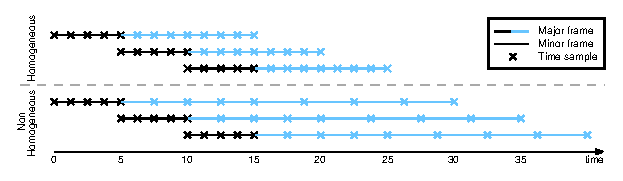
\includegraphics[width=1.0\textwidth]{non_homogeneous_control.eps}
\caption{Receding horizon planning}
\label{fig:multiplan}
\end{figure*}


\begin{figure*}[t!]
\centering
%  trim={<left> <lower> <right> <upper>}
\subfigure[]{
\label{subfig:network1}
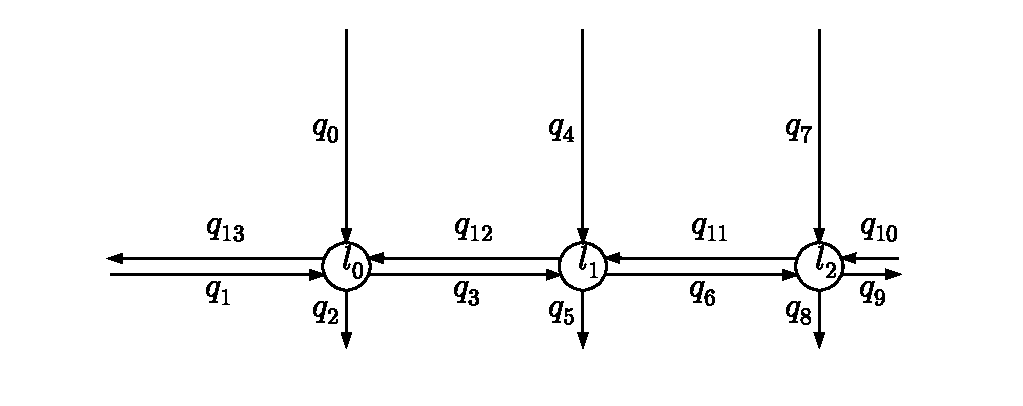
\includegraphics[width=0.45\textwidth]{network_3_lights}}
\subfigure[]{
\label{subfig:network2}
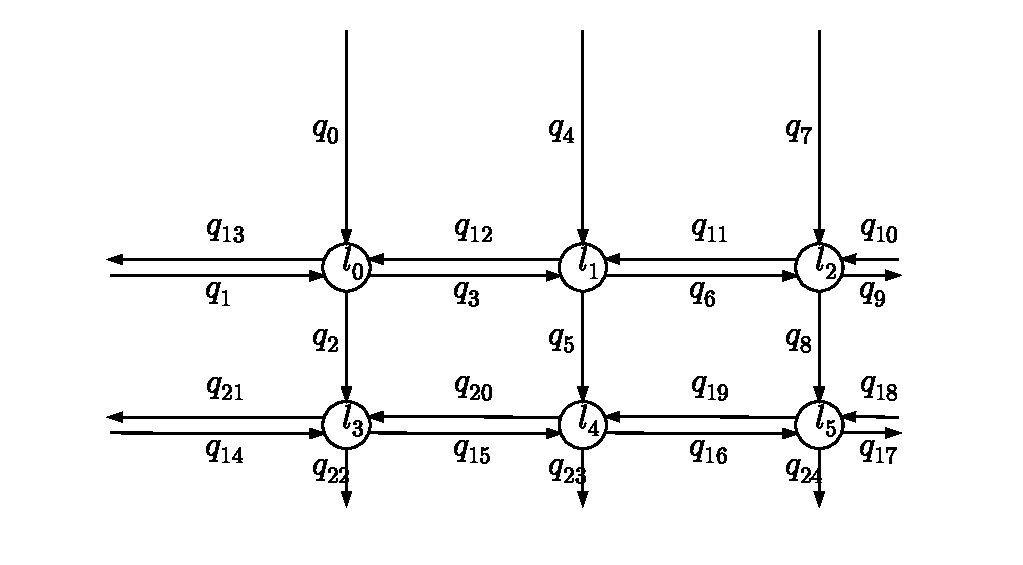
\includegraphics[width=0.45\textwidth]{network_6_lights}}
\subfigure[]{
\label{subfig:network3}
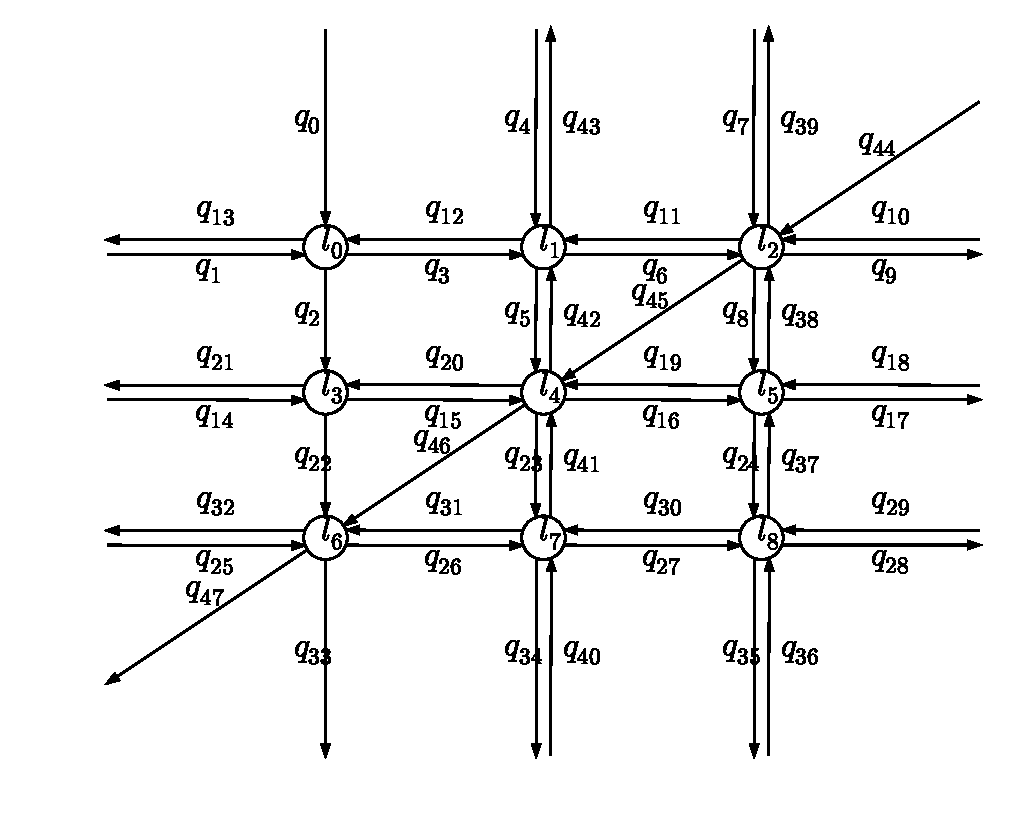
\includegraphics[width=0.45\textwidth]{network_9_lights}}
\caption{Networks used to evaluate the QTM performance.}
\label{fig:networks}
\end{figure*}

\begin{table}[h]
\caption{Network Demand Profiles (vehicles per second)}
\label{tab:network_demand}
\centering
\begin{tabular}{cccccc}
\toprule
& Inflow Queues & 0 - 55 s & 55 - 70 s & 70 - 85 s & > 85 s\\
\midrule
\multirow{2}{*}{Network 1}&$q_0$ & 1 & 1 & 1 & 0 \\
&$q_4, q_7$ & 4 & 4 & 4 & 0 \\
&$q_1,q_{10}$& 2 & 4 & 2 & 0 \\
\midrule
\multirow{2}{*}{Network 2}&$q_0$ & 1 & 1 & 1 & 0 \\
&$q_4,q_7,q_{14}$& 4 & 4 & 4 & 0 \\
&$q_1, q_{10},q_{18}$ & 2 & 4 & 2 & 0 \\
\midrule
\multirow{2}{*}{Network 3}&$q_0$ & 1 & 1 & 1 & 0 \\
&$q_4,q_7,q_{14},q_{25},$& 4 & 4 & 4 & 0 \\
&$q_1, q_{10},q_{18},q_{29},q_{36},q_{40},q_{44}$ & 2 & 4 & 2 & 0 \\
\bottomrule\\
\end{tabular}
\end{table}




%\begin{table}[h]
%\caption{Network 3 traffic parameters}
%\label{tab:net3wave}
%\centering
%\begin{tabular}{cccccc}
%\toprule
%Queue & Background & End & Wave & Start &End\\ 
%\midrule
%$q_0$ & 1 & 85 & 1 & 55 & 70\\
%$q_1$ & 2 & 85 & 4 & 55 & 70\\
%$q_4$ & 4 & 85 & 4 & 55 & 70\\
%$q_7$ & 4 & 85 & 4 & 55 & 70\\
%$q_{10}$ & 2 & 85 & 4 & 55 & 70\\
%$q_{14}$ & 4 & 85 & 4 & 55 & 70\\
%$q_{18}$ & 2 & 85 & 4 & 55 & 70\\
%$q_{25}$ & 4 & 85 & 4 & 55 & 70\\
%$q_{29}$ & 2 & 85 & 4 & 55 & 70\\
%$q_{36}$ & 2 & 85 & 4 & 55 & 70\\
%$q_{40}$ & 2 & 85 & 4 & 55 & 70\\
%$q_{44}$ & 2 & 85 & 4 & 55 & 70\\
%\bottomrule\\
%\end{tabular}
%\end{table}

\subsection{Results}

We compare the performance of non-homogeneous and homogeneous solutions in two
ways: comparing the decrease in total travel time with increasing major frame
time (greater look ahead), and analysing the distribution of delay in each queue
of the network.
\cref{subfig:travel_time_3,subfig:travel_time_6,subfig:travel_time_9} show a
comparison between the number of time samples\fnremark{FWT: This is the first
time we mention time samples, so we need to relate it with the \DT[]'s and
major frame or use something defined previously.} used in the major frame vs the
\% improvement in total travel time, where 0\% is the reference solution total
travel time. It can be seen that for all three networks, using a non-homogeneous
$\DT[]$ converges towards the optimum total travel time more quickly than the
homogeneous $\DT[]$.\toIain{We need to explain that as $N$ increases, the size
of the major frame increases but for a given $N$ the major frame size between
homogeneous and non-homogeneous is different. What is this relation for the
non-homogeneous \DT[]?} 

\cref{subfig:delay_3,subfig:delay_6,subfig:delay_9} show the distribution of the
total delay observed by each car while traversing the network for different
solutions. This gives us an indication of the quality of the solution in terms
of the number of vehicles that experience significant delay and if the solution
may be starving some parts of the network.  Each group of box plots represents a
different number of time samples: when the non-homogeneous $\DT[]$ first converges to
the optimum solution; when the homogeneous $\DT[]$ first converges on the
optimum solution; and the optimum solution itself. With all three networks the
quality of the solution is better or  the same using a non-homogeneous $\DT[]$
compared to a homogeneous $\DT[]$ with the same number of sample
points.\fnremark{FWT: we need to define what we mean by better, for instance,
smaller 75\% quartile and max delay.}

Finally, \cref{fig:cumu} shows the cumulative arrival and departure curves and
the how delay evolves over time for $q_1$ of network 2.  \cref{subfig:cumu1}
shows the comparison at the point where the non-homogeneous $\DT[]$ first
converges and shows that with the longer major frame time of the
non-homogeneous $\DT[]$, the solver is able to find a coordinated signal policy
along the avenue to dissipate the extra traffic that arrives at the 55s point,
while the homogeneous $\DT[]$ with its shorter major frame \remark{fails to find
a coordinated policy along the avenue and experiences more delay}.\toIain{I
don't think that failure to coordinate is the best way to describe it because
there is coordination but it happens too late.} Once the homogeneous $\DT[]$ has
converged in \cref{subfig:cumu2}, both solutions are close to the optimum
solution which is shown in \cref{subfig:cumu3}.

\begin{figure*}[t!]
\centering

%  trim={<left> <lower> <right> <upper>}
\subfigure[]{
\label{subfig:travel_time_3}
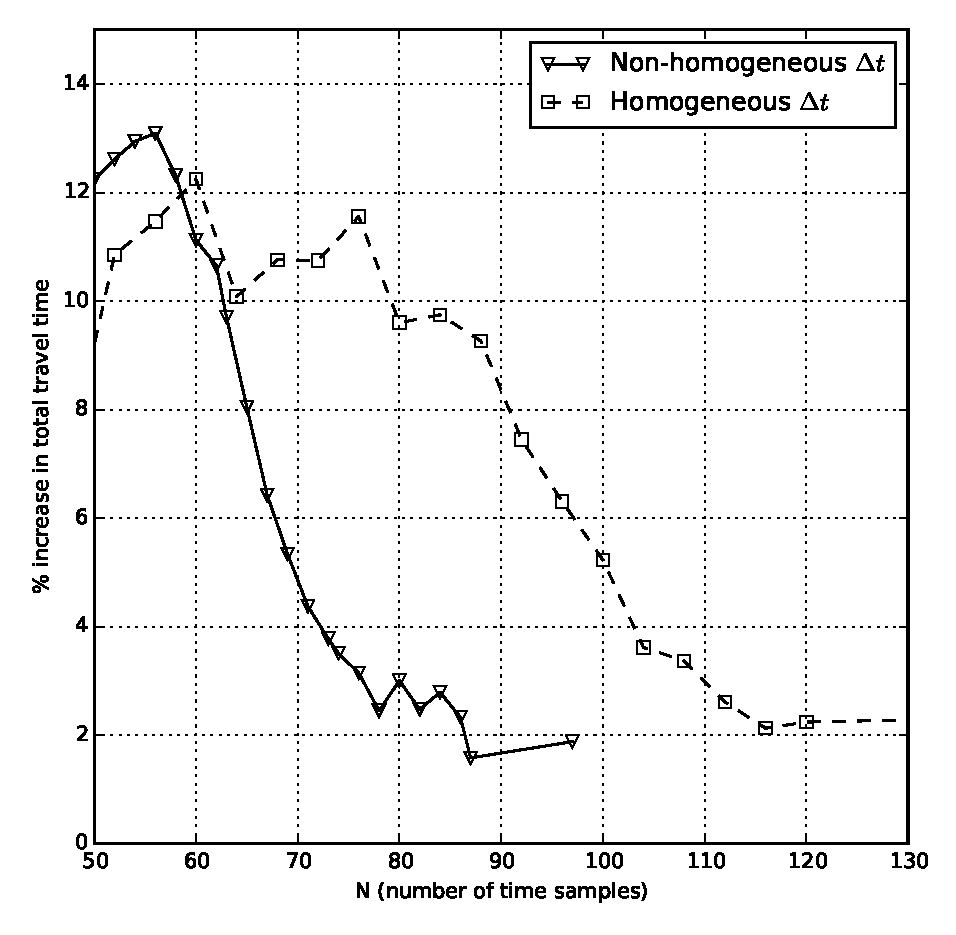
\includegraphics[width=0.4\textwidth]{samples_plot_3_lights}}
\subfigure[]{
\label{subfig:delay_3}
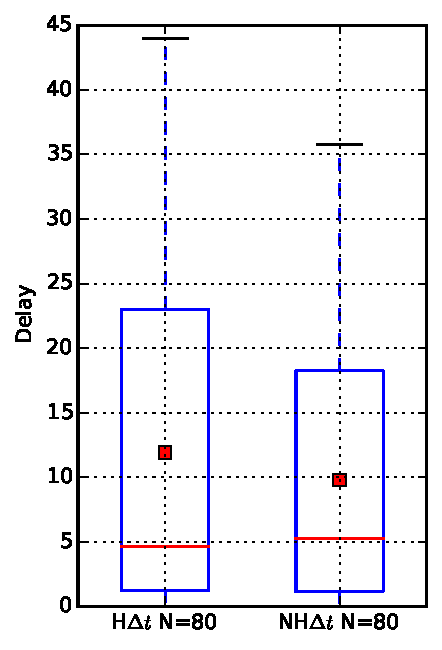
\includegraphics[keepaspectratio,height=0.3\textwidth]{box_plot_early_3l.pdf}
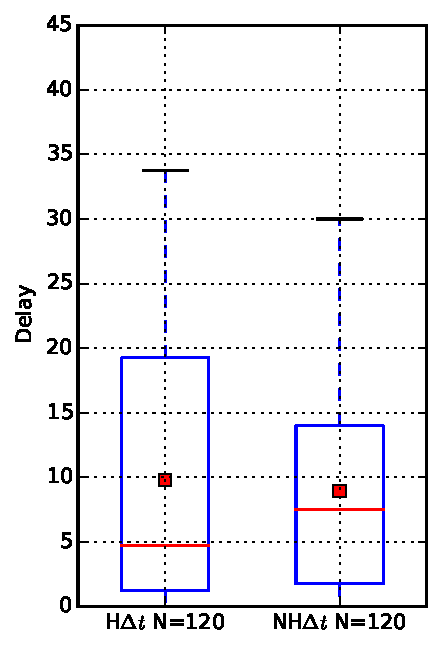
\includegraphics[keepaspectratio,height=0.3\textwidth]
{box_plot_converg_3l.pdf}
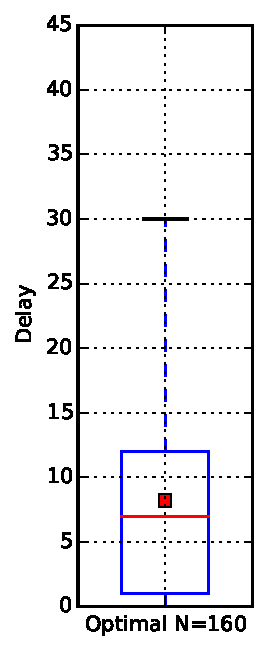
\includegraphics[keepaspectratio,height=0.3\textwidth]{box_plot_final_3l.pdf}}

\subfigure[]{
\label{subfig:travel_time_6}
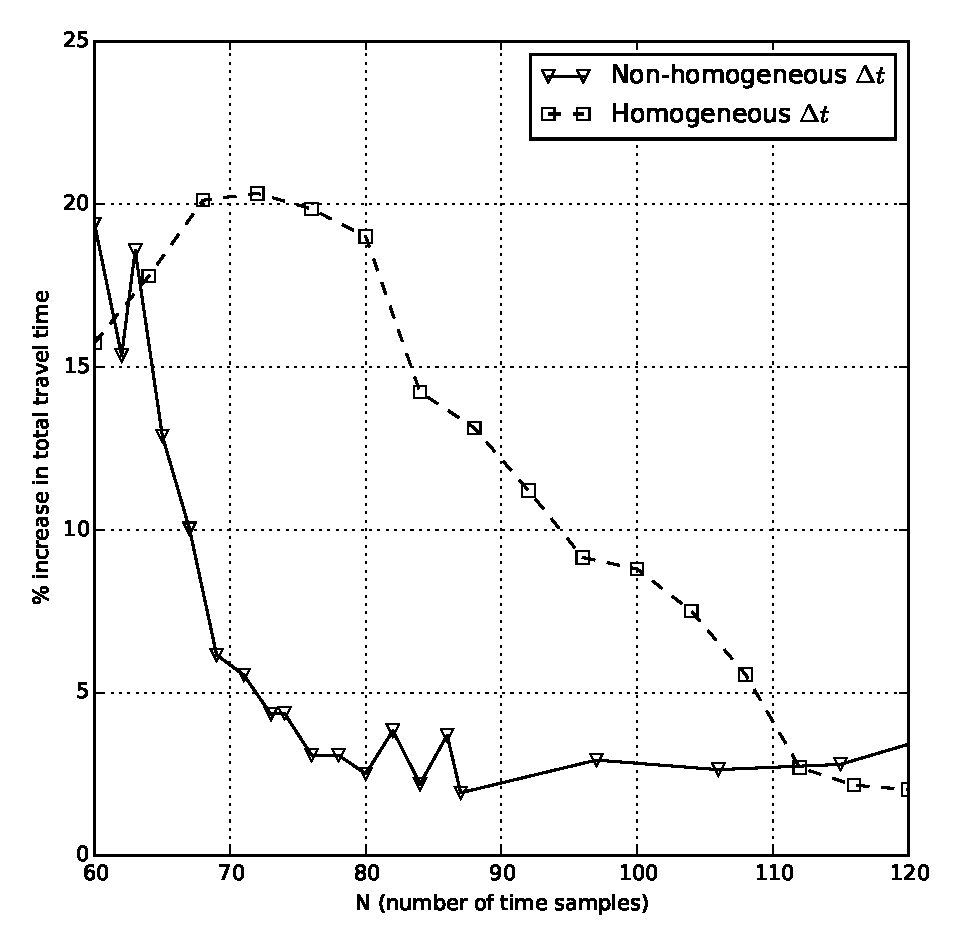
\includegraphics[width=0.4\textwidth]{samples_plot_6_lights}}
\subfigure[]{
\label{subfig:delay_6}
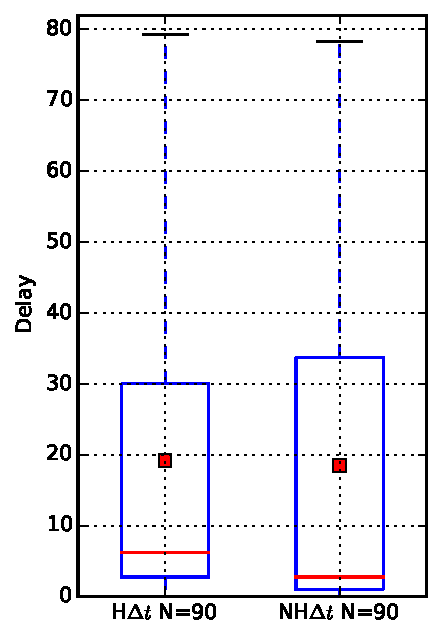
\includegraphics[keepaspectratio,height=0.3\textwidth]{box_plot_early_6l.pdf}
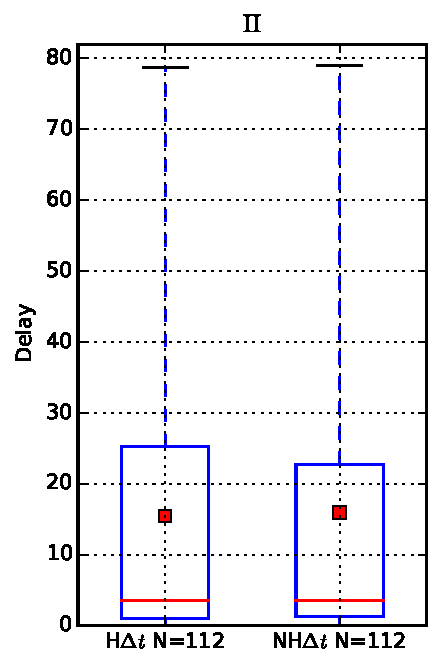
\includegraphics[keepaspectratio,height=0.3\textwidth]
{box_plot_converg_6l.pdf}
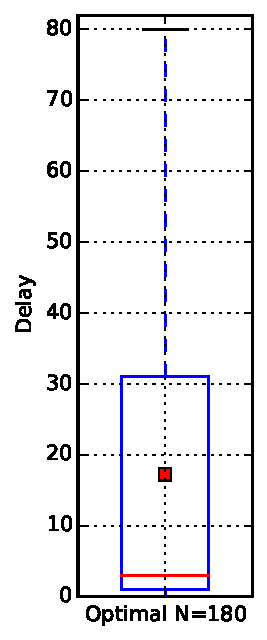
\includegraphics[keepaspectratio,height=0.3\textwidth]{box_plot_final_6l.pdf}}

\subfigure[]{
\label{subfig:travel_time_9}
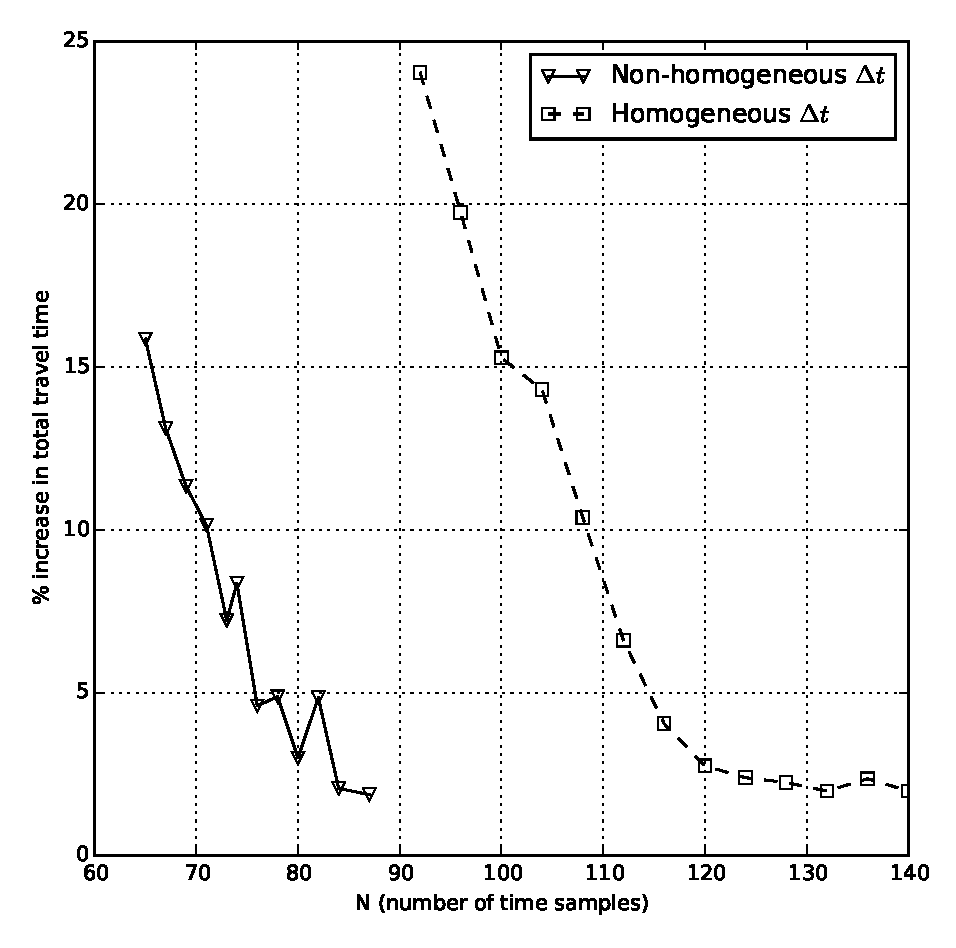
\includegraphics[width=0.4\textwidth]{samples_plot_9_lights}}
\subfigure[]{
\label{subfig:delay_9}
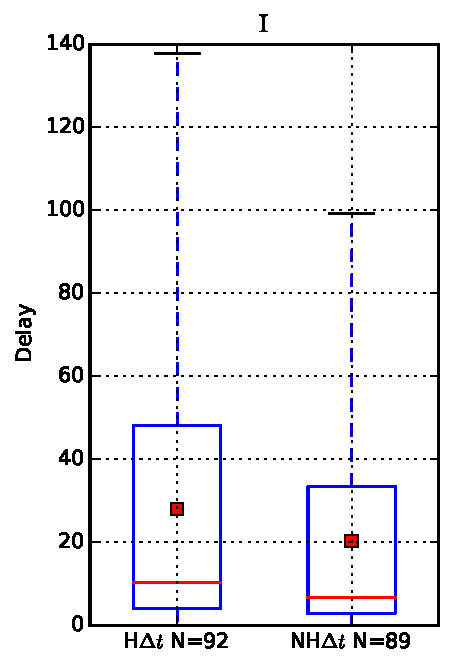
\includegraphics[keepaspectratio,height=0.3\textwidth]{box_plot_early_9l.pdf}
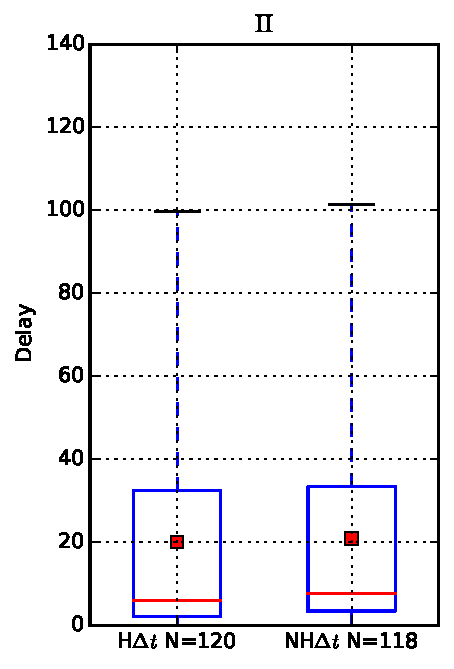
\includegraphics[keepaspectratio,height=0.3\textwidth]
{box_plot_converg_9l.pdf}
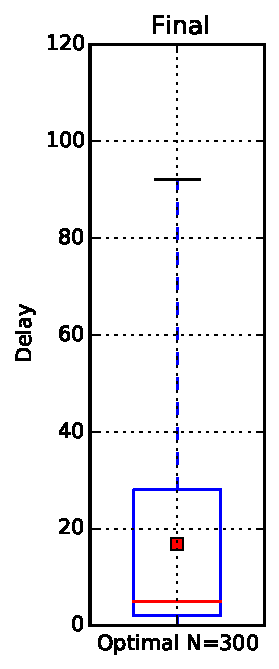
\includegraphics[keepaspectratio,height=0.3\textwidth]{box_plot_final_9l.pdf}}
\caption{Results for the three networks showing the comparitive \% increase in 
total travel time for the network between using a homogeneous $\DT[]$ and a 
non-homogeneous $\DT[]$, and the 
distribution of delay time at the convergence point of non-homogeneous $\DT[]
$, the convergence point of homogeneous $\DT[]$ and for the fully solved 
optimal solution. (a) and (b) 3 light avenue, 
(c) and (d) 6 light grid, and (e) and (f) 9 light grid,}
\label{fig:results}
\end{figure*}

\begin{figure*}[t!]
\centering

%  trim={<left> <lower> <right> <upper>}
\subfigure[]{
\label{subfig:cumu1}
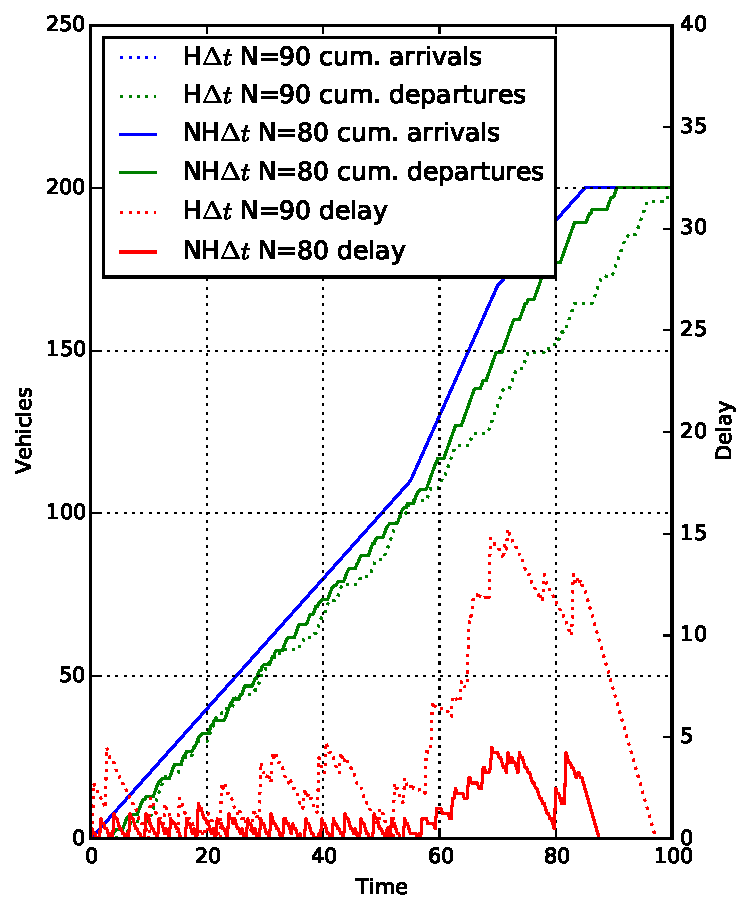
\includegraphics[width=0.32\textwidth]{cum_plot_early_6l.pdf}}
\subfigure[]{
\label{subfig:cumu2}
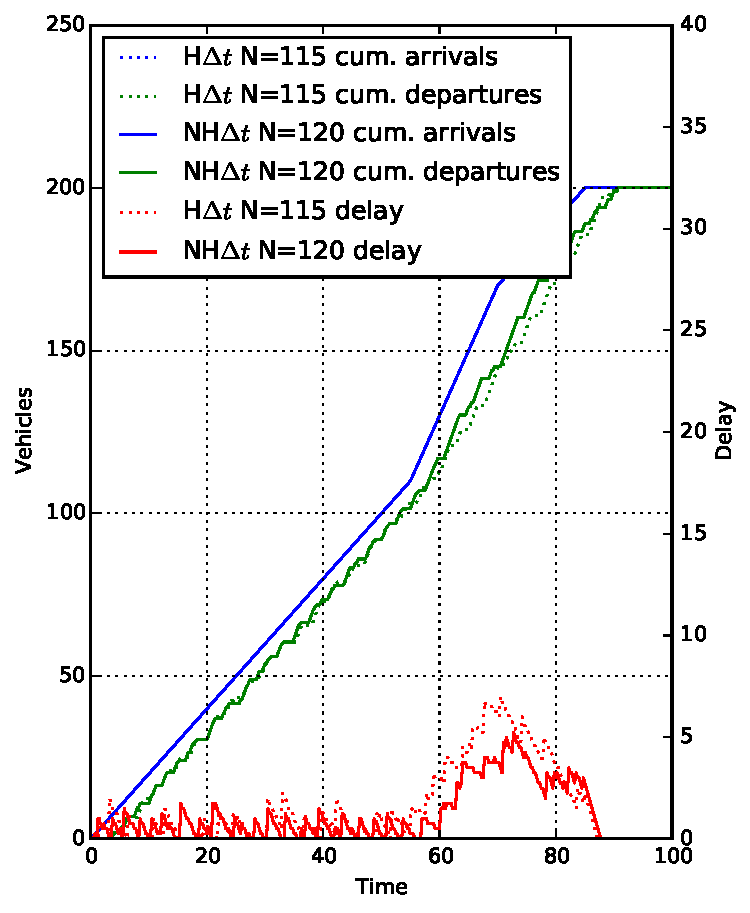
\includegraphics[width=0.32\textwidth]{cum_plot_converg_6l.pdf}}
\subfigure[]{
\label{subfig:cumu3}
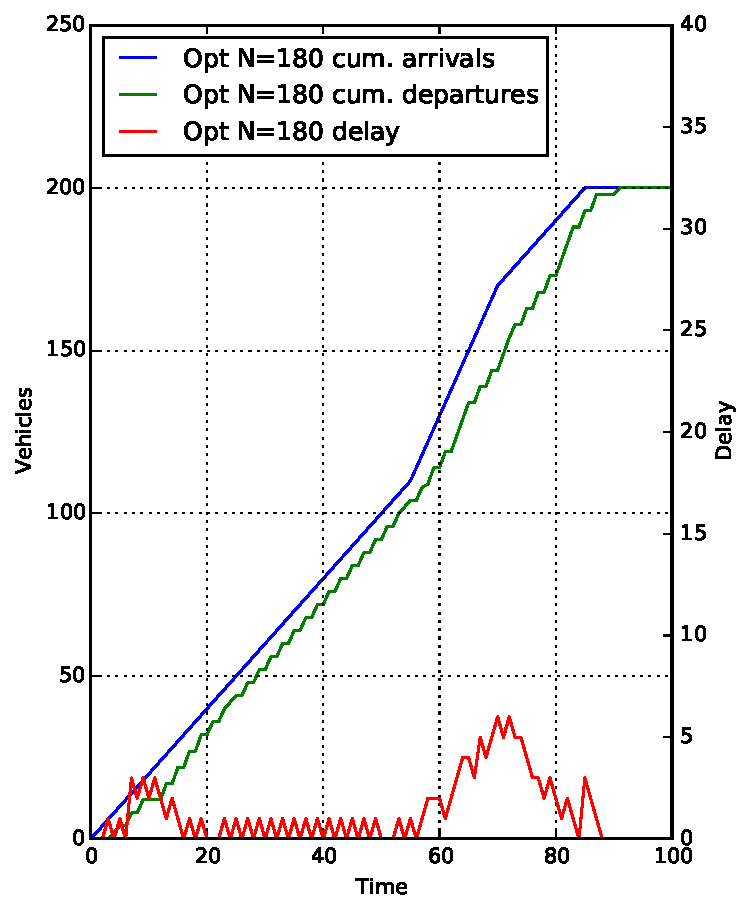
\includegraphics[width=0.32\textwidth]{cum_plot_final_6l.pdf}}
\caption{Cumulative arrival and departure curves and delay for queue 1 in the 6 
light grid. (a) at the convergence point of the non-homogeneous $\DT[]$ it is 
near to the optimum solution while 
homogeneous $\DT[]$ lags behind (b) at the convergence point of 
homogeneous $\DT[]$ both are near optimum, and (c) the fully solved optimal 
solution}
\label{fig:cumu}
\end{figure*}

